\section{Excercise CarRentalStructs}
\label{sec:car_rental_structs}

\subsection*{Add the Attributes to Structs}
After adding the attributes from the entity diagram to the 
\texttt{.../golang/CarRental/CarRentalStructs/CarRentalStructs.go} path and saving
the IDE automatically formats the code and indents it correctly.

\subsection*{Initialize and Print Structs}
The result of the initialization and printing of the structs is shown in figure \ref{fig:car_rental_structs}.
\begin{figure}[H]
    \centering
    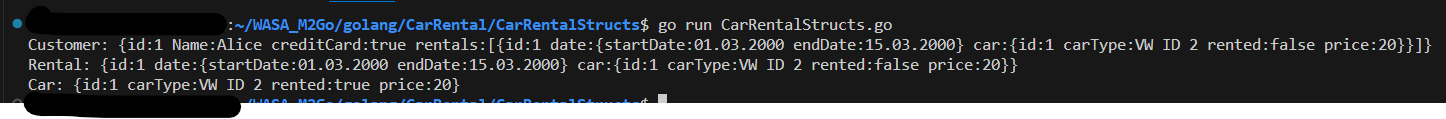
\includegraphics[width=\textwidth]{figures/goLang/carRental/carRental_structs.png}
    \caption{Output of the structs}
    \label{fig:car_rental_structs}
\end{figure}

\subsection*{Create an Array of Rentals}
The function works as follows:
\begin{enumerate}
    \item The array \texttt{cartypes} holds the string of 5 different cartypes
    \item The function \texttt{createRentals(id, date, car)} returns 5 rentals that are appended to the array
    \item Via \texttt{fmt.Println(rentals)} the array is printed into the console
\end{enumerate}

The result is shown in figure \ref{fig:car_rental_array_five_rentals}.
\begin{figure}[H]
    \centering
    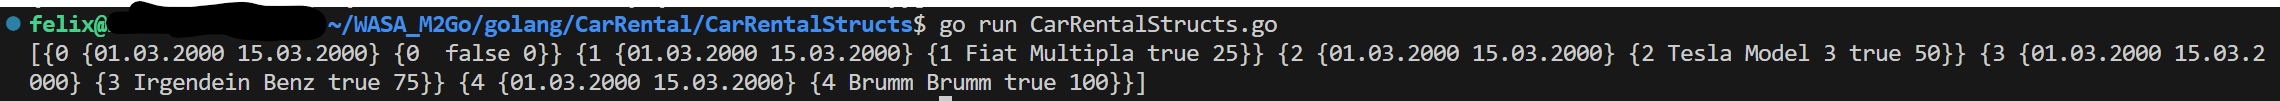
\includegraphics[width=\textwidth]{figures/goLang/carRental/carRental_arrayFiveRentals.png}
    \caption{Output of the Array of Rentals}
    \label{fig:car_rental_array_five_rentals}
\end{figure}

\section{Excercise CarRentalTests}
\subsection*{Analyze OCL Constraints}
In the given task five invariants are described.
These invariants are implemented in \texttt{./CarRentalTests/CarRentalTests.go} and executed in \texttt{./CarRentalStructs/CarRentalStructs.go}.
\begin{enumerate}
    \item \texttt{self.Date.Year >= 2000}: CarRentalTests.go line 20-22
    \item \texttt{self.Date.Month < 13}: CarRentalTests.go line 24-26
    \item \texttt{self.Date.Moth >= 1}: CarRentalTests.go line 24-26
    \item \texttt{self.ValidateNumberOfDaysInMonth() == True}: CarRentalTests.go line 32
\end{enumerate}

\subsection*{Run Test}
After running the test function an error occurs. 
The test, therefore, does not pass.
The error is shown in figure \ref{fig:car_rental_test_error}.

This error is caused due to a false implementation in line 20 of \texttt{./CarRentalTests/CarRentalTests.go}
In the first test, it checks if the year is $>2000$, yet for correct execution it needs to be $>=2000$.

\begin{figure}[H]
    \centering
    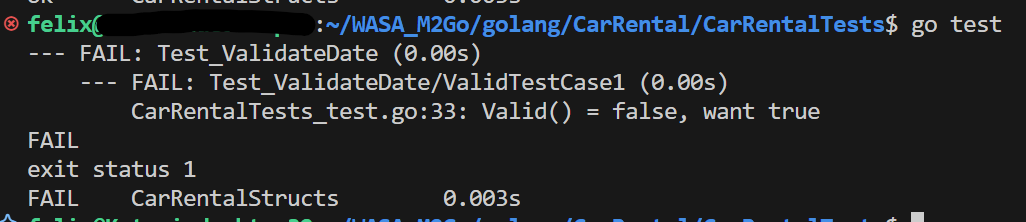
\includegraphics[width=0.8\textwidth]{figures/goLang/carRental/carRental_dateTestError.png}
    \caption{Error of the Test}
    \label{fig:car_rental_test_error}
\end{figure}

\subsection*{Correct Code}
As mentioned in the subsection above, line 20 is not implemented correctly.
By changing line 20 from \texttt{if !(d.Year \> 2000)} to \texttt{if !(d.Year \>\= 2000)} the code will execute correctly and the test passes.
The working tree of the changes is shown in figure \ref{fig:car_rental_test_working_tree}.

\begin{figure}[H]
    \centering
    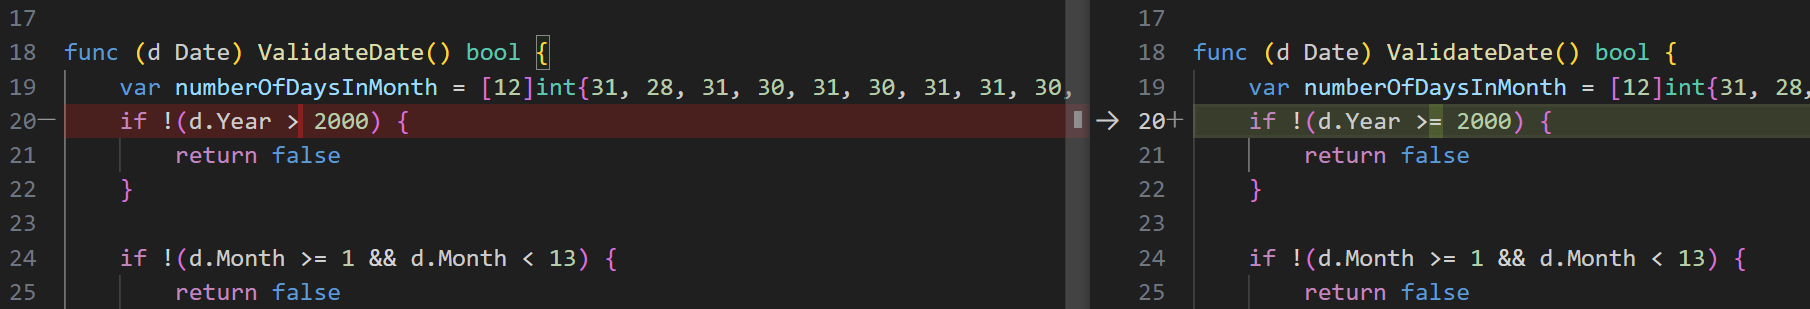
\includegraphics[width=\textwidth]{figures/goLang/carRental/carRental_dateTestWorkingTree.png}
    \caption{Working Tree of the Changes}
    \label{fig:car_rental_test_working_tree}
\end{figure}

\subsection*{Negative Test Case}
Implementing an invalid test-case the following code is added to the test function:
\begin{lstlisting}[
    language=Golang,
    numbers=left,
    numberstyle=\tiny,
    caption={Invalid Test Case},
    label={lst:invalid_test_case}
    ]
	    name:   "InvalidTestCase1",
        fields: fields{Day: 12, Month: 13, Year: 2000},
	    want:   false,  
\end{lstlisting}

As shown in listing \ref{lst:invalid_test_case} the month is set to 13, which is invalid.
Therefore the test should return false.
The test, however, runs succesfully due to the want value set to false.
